% !TEX program = xelatex
\documentclass[20pt, a4paper]{article}
\usepackage{listings}
\usepackage{hyperref}
\usepackage{plantuml}
\usetikzlibrary{arrows, shapes, automata, petri, positioning, calc}
\usepackage{graphicx}
\usepackage{ragged2e}
\usepackage{color}
\usepackage{xepersian}
\usepackage{subfiles}
\settextfont[Scale=1]{XB Roya}
\renewcommand{\baselinestretch}{1.5}

\begin{document}
\centerline{پایگاه داده پیشرفته}
\centerline{دکتر شجاعی مهر}
\centerline{علیرضا سلطانی نشان}
\centerline{\today}

\tableofcontents

\newpage

\section{مفاهیم}

\subsection{تراکنش}

تراکنش واحد اجرای برنامه است. عملیاتی که در هر تراکنش می‌تواند شامل شود موارد
زیر می‌باشد:

\begin{itemize}
    \item Create
    \item Read
    \item Update
    \item Delete
\end{itemize}

\subsection{قوانین \lr{ACID}}

\subsubsection{اتمیک یا \lr{Atomicity}}

هر تراکنش دیتابیس به صورت اتمیک می‌باشد. این قضیه بدان معناست که این تراکنش یا
باید کاملا انجام شود یا کلا لغو و صرف نظر شود. در غیر این صورت اگر تراکنش به
صورت ناتمام و ناقص انجام شود عواقب مختلفی روی دیتابیس خواهد گذاشت.

\subsubsection{جامعیت یا \lr{Consistency}}

هر تراکنش باید از قوانین جامعیت پیروی کند. نمی‌توان داده یا را وارد جدولی از
دیتابیس کرد که به صورت معتبر نباشد. در برخی از مراجع این قانون را به اجرای صحیح
و سازگار تراکنش می‌شناسند. مهم ترین مثال آن است که شما یک \lr{Validation} روی یک
مقداری از فیلد جدول تنظیم می‌کنید که هر داده‌ای بر روی آن فقط با شرایط تعریف شده
بایستی وارد شود.

خالی از لطف نیست که در مورد مرجع پذیری داده‌ها در این قسمت نیز می‌توان صحبت کرد
تا بتواند قوانین جامعیت را به طور صحیح کامل کرد. مرجع پذیری زمانی مطرح می‌شود که
یک رکوردی از داده وقتی وارد جدولی از دیتابیس می‌شود ممکن است ارتباط مشخصی با
جدولی دیگر داشته باشد. پس به همین خاطر کلید‌های اصلی و خارجی در خصوص جامعیت وجود
دارند که داده‌ای معنادار را پس از پرس و جو از دیتابیس به برنامه نویس برگرداند.
یادآوری، بخش جوین‌ها در دیتابیس و تعریف رفرنس در هنگام تعریف کلید جانبی.

\subsubsection{انزوا یا \lr{Isolation}}

هر سیستم جامع پایگاه داده‌ای باید بتواند روی همروند تراکنش‌ها مدیریت و کنترل
کامل داشته باشد. انزوا تراکنش‌ها قابلیت کنترل و تنظیم بر اساس \lr{DBMS} است.

به طور کل همروندی یا همزمانی به حالتی گفته می‌شود که چند تراکنش بخواهند در یک
زمان به صورت موازی روی یک منبع عملیات خواندن و نوشتن را انجام دهند. اما این
عملیات به طور کل هزینه خاص و مشخصی برای برنامه نویس و مدیر دیتابیس دارد.

\subsubsection{قابلیت اعتماد یا \lr{Duribility}}

قابلیت اعتماد یکی از مهم‌ترین ویژگی‌های هر سیستم دیتابیسی است. یعنی بتوان
داده‌ها را در پایگاه‌داده به صورت پایدار و ثابت نگهداری و مراقبت کرد. در صورت
بروز مشکل روی داده‌های یک دیتابیس می‌توان به عملیات انجام شده در این قسمت مراجعه
کرد. بطور کلی این بخش قابلیت کنترل و مدیریت دارد و می‌توان مجموعه فرایند‌های
نگهداری و بک‌آپ را به صورت خودکار انجام داد.

\subsection{تنظیم قابلیت انزوا}

انزوا و مدیریت همروندی در دیتابیس به چهار طریق قابل انجام است:

\begin{enumerate}
    \item \lr{Read uncommitted}
    \item \lr{Read commmitted} 
    \item \lr{Repeadable read}
    \item \lr{Serializable}
\end{enumerate}

یادآوری: هر تراکنش دو حالت در پایان پیدا می‌کند:

\begin{itemize}
    \item \lr{Commit}: تراکنش درنهایت تایید و انجام می‌شود
    \item \lr{Abort}: تراکنش در نهایت سقط یا صرفه نظر می‌شود
\end{itemize}

\subsubsection{وضعیت تراکنش}


نکته: \lr{Abort} در دو شرط اتفاق می‌افتد:

\begin{enumerate}
    \item زمانی که اجرای تراکنش به خطای \lr{Run time} دچار شود.
    \item خرابی و نقص سیستم که روی اجرای تراکنش تاثیر می‌گذارد که کامل نشود
\end{enumerate}

\begin{figure}
    \centering
    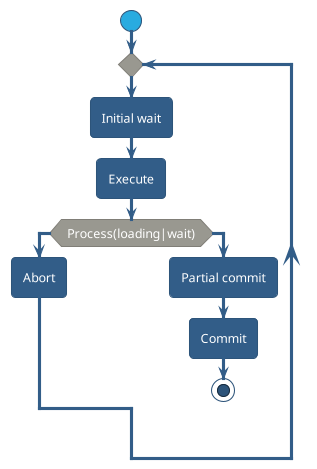
\includegraphics[width=0.5\textwidth]{umls/transactionStatus.png}
    \caption{نمودار شروع فرایند تراکنش‌ها}
    \label{fig: uml}
\end{figure}

\newpage

\subsection{همروندی}

\subsection{مزیت همروندی}

\begin{enumerate}
    \item افزایش سرعت گذردهی یا \lr{throughput}
    \item کاهش میانگین زمان پاسخدهی به تراکنش مورد نظر
\end{enumerate}

\subsection{معایب همروندی} 

\begin{enumerate}
    \item \lr{Last update}: تغییرات گمشده به دلیل همزمانی در خواندن و نوشتن
    قانون \lr{Write before Write}
    \item \lr{Uncommitted}: خواندن داده‌ای که معتبر نیست. معمولا به آن \lr{Dirty
    read} هم گفته می‌شود. قانون \lr{Write before Read}
    \item \lr{Inconsistent retrieval}: بازیابی داده‌ای که ناهمگان است. \lr{Read
    before Write}
\end{enumerate}

\subsection{زمان‌بندی}

زمان‌بندی به اجرای همروند و همزمان چندین تراکنش با هم گفته می‌شود.

\subsection{نظریه پی در پی پذیری زمان‌بندی‌ها}

به دو روش می‌توان به پی در پی پذیری رسید:

\begin{enumerate}
    \item \lr{Conflict serializablity}
    \item \lr{View serializablity}
\end{enumerate}

نماد‌های مورد استفاده برای تعریف تراکنش‌ها:

\begin{itemize}
    \item $R_{i}| Q |$
    \item $W_{i}| Q |$
    \item $C_{i}| Q |$
    \item $A_{i}| Q |$
    \item $B_{i}| Q |$
    \item $E_{i}| Q |$
\end{itemize}

\subsection{سه شرط اصلی تصادم}

اگر $p_{i}$ و $q_{j}$ دو تراکنش باشند:

\begin{enumerate}
    \item \lr{i != j}
    \item هر دو به یک داده دسترسی داشته باشند
    \item حداقل یکی از دستورات عمل نوشتن یا \lr{write} داشته باشد
\end{enumerate}


\begin{LTR}
    \begin{table}[h]
        \centering
        \begin{RTL}
            \caption{حالات تصادم}
        \end{RTL}
        \begin{tabular}{|c|c|c|}
            \hline
            & $R_{i}(Q)$ & $W_{j}(Q)$ \\ \hline
            $R_{i}(Q)$ & ندارد &  دارد  \\ \hline
            $W_{j}(Q)$ & دارد & دارد  \\ \hline
        \end{tabular}
    \end{table}
\end{LTR}

\subsection{زمان‌بندی سریالی}

در زمان‌بندی پی در پی، زمانی که یک تراکنش \lr{commit} یا \lr{abort} شود به دنبال
تراکنش بعدی خواهد رفت که به آن تراکنش سریالی یا \lr{Serializable schedule}
می‌گویند.

\begin{LTR}
  \lr{$S_{1} = R_{1}(A) W_{1}(A) a_{1} W_{2}(A) W_{2}(B) C_{2}$}
\end{LTR}

زمان‌بندی سریالی بالا در حقیقت به دو فرایند تقسیم می‌شود. چرا که در انتهای
تراکنش اول پیام سقوط کرده و برنامه به دنبال فرایند بعدی رفته است که روی منبع
دیگری در حال انجام پردازش است.

فرایند نافرجام اول:

\begin{LTR}
  \lr{$S_{1} = R_{1}(A) W_{1}(A) a_{1}$}
\end{LTR}

فرایند \lr{commit} شده دوم:

\begin{LTR}
  \lr{$S_{1} = W_{2}(A) W_{2}(B) C_{2}$}
\end{LTR}

\begin{LTR}
    \begin{table}[h]
        \centering
        \begin{RTL}
            \caption{تراکنش‌های سریالی پی در پی}
        \end{RTL}
        \begin{tabular}{|c|c|c|c|c|c|c|}
            \hline
            $T_{1}$ & $R_{1}(A)$ & $W_{1}(A)$ & $a_{1}$ & & & \\ \hline
            $T_{2}$ & & & & $W_{2}(A)$ & $W_{2}(B)$ & $C_{2}$ \\ \hline
        \end{tabular}
    \end{table}
\end{LTR}

\subsection{زمان‌بندی‌های معادل در برخورد}

زمانی که دستورات یک زمان‌بندی را وارد زمانبندی دیگر کنیم به گونه‌ای که باعث تصادم
و برخورد نشود، این دستورات در این زمان‌بندی با هم معادل در برخورد هستند.

با توجه به تراکنش‌های \lr{$t_{1}$} و \lr{$t_{2}$} و \lr{$t_{3}$} و \lr{$t_{4}$}
زیر، می‌توان دریافت که این دو تراکنش با یکدیگر معادل در برخورد هستند. به گونه‌ای
که بعد از برخورد هیچ تصادمی رخ نداده است.

\begin{LTR}
    \begin{table}[h]
        \centering
        \begin{RTL}
            \caption{تراکنش‌های معادل در برخورد اول}
        \end{RTL}
        \begin{tabular}{|c|c|c|c|c|c|c|c|c|c|c|}
            \hline
            $T_{1}$ & $R(Q)$ & $W(Q)$ & & $R(P)$ & & $W(P)$ & $C$ & & & \\ \hline
            $T_{2}$ & & & $R(Q)$ & & $W(Q)$ & &  & $K(Q)$ & $W(Q)$ & $C$ \\ \hline
        \end{tabular}
    \end{table}
\end{LTR}

\begin{LTR}
    \begin{table}[h]
        \centering
        \begin{RTL}
            \caption{تراکنش‌های معادل در برخورد دوم}
        \end{RTL}
        \begin{tabular}{|c|c|c|c|c|c|c|c|c|c|c|}
            \hline
            $T_{3}$ & $R(Q)$ & $W(Q)$ & & $R(P)$ & $W(P)$ & & $C$ & & & \\ \hline
            $T_{4}$ & & & $R(Q)$ & & & $W(Q)$ &  & $K(Q)$ & $W(Q)$ & $C$ \\ \hline
        \end{tabular}
    \end{table}
\end{LTR}

\newpage

اما در مثال بعد هر دو تراکنش \lr{$t_{1}$} و \lr{$t_{2}$} مستعد به برخورد در یکی
از فرایند‌ها در زمان هستند.

\begin{LTR}
    \begin{table}[h]
        \centering
        \begin{RTL}
            \caption{تراکنش‌های معادل در برخورد اول}
        \end{RTL}
        \begin{tabular}{|c|c|c|c|c|c|c|c|c|c|c|}
            \hline
            $T_{1}$ & $R(Q)$ & $W(Q)$ & & $R(P)$ & & $W(P)$ & $C$ & & & \\ \hline
            $T_{2}$ & & & $R(Q)$ & & $W(Q)$ & &  & $K(Q)$ & $W(Q)$ & $C$ \\ \hline
        \end{tabular}
    \end{table}
\end{LTR}


\begin{LTR}
    \begin{table}[h]
        \centering
        \begin{RTL}
            \caption{تراکنش‌های معادل در برخورد اول}
        \end{RTL}
        \begin{tabular}{|c|c|c|c|c|c|c|c|c|c|c|}
            \hline
            $T_{1}$ & $R(Q)$ & $W(Q)$ & & $R(P)$ & & $W(P)$ & $C$ & & & \\ \hline
            $T_{2}$ & & $R(Q)$ & $R(Q)$ & & $W(Q)$ & &  & $K(Q)$ & $W(Q)$ & $C$ \\ \hline
        \end{tabular}
    \end{table}
\end{LTR}

\end{document}